%%%%%%%%%%%%%%%%%%%%%%%%%%%%%%%%%%%%%%%%%%%%%%%%%%%%%%%%%%%%%%%%
%                                                              %
%                                                              %
% Macallyster S. Edmondson                                     %
%                                                              %
% ECE351-53                                                    %
%                                                              %
% Lab #8                                                       %
%                                                              %
% 03/22/2022                                                   %
%                                                              %
% Straightforward layout, broken into sections, uses many      %
% common libraries. Note, Hyperlinks are not highlighted.      %
%                                                              %
%%%%%%%%%%%%%%%%%%%%%%%%%%%%%%%%%%%%%%%%%%%%%%%%%%%%%%%%%%%%%%%%

%%%%%%%%%%%%%%%%%%%%%%%%%%%%%%%%%%%%%%%%%%%
%%% DOCUMENT PREAMBLE %%%
\documentclass[12pt]{report}
\usepackage[english]{babel}
%\usepackage{natbib}
\usepackage{url}
\usepackage[utf8x]{inputenc}
\usepackage{amsmath}
\usepackage{graphicx}
\graphicspath{{./images/}}
\usepackage{parskip}
\usepackage{fancyhdr}
\usepackage{vmargin}
\usepackage{listings}
\usepackage[hidelinks]{hyperref}
\usepackage{xcolor}
\usepackage[nodayofweek]{datetime}
\usepackage[section]{placeins}
\usepackage{pdfpages}
\usepackage{float}
\definecolor{codegreen}{rgb}{0,0.6,0}
\definecolor{codegray}{rgb}{0.5,0.5,0.5}
\definecolor{codeblue}{rgb}{0,0,0.95}
\definecolor{backcolour}{rgb}{0.95,0.95,0.92}
\lstdefinestyle{mystyle}{
backgroundcolor=\color{backcolour},
commentstyle=\color{codegreen},
keywordstyle=\color{codeblue},
numberstyle=\tiny\color{codegray},
stringstyle=\color{codegreen},
basicstyle=\ttfamily\footnotesize,
breakatwhitespace=false,
breaklines=true,
captionpos=b,
keepspaces=true,
numbers=left,
numbersep=5pt,
showspaces=false,
showstringspaces=false,
showtabs=false,
tabsize=2
}
\lstset{style=mystyle}
\setmarginsrb{3 cm}{2.5 cm}{3 cm}{2.5 cm}{1 cm}{1 cm}{1 cm}{1.5 cm}
\title{Lab \#9 Report}
% Title
\author{Macallyster S. Edmondson}
% Author
\newdate{date}{29}{03}{2022}
\date{\longdate\displaydate{date}}
% Date
\makeatletter
\let\thetitle\@title
\let\theauthor\@author
\let\thedate\@date
\makeatother
\pagestyle{fancy}
\fancyhf{}
\rhead{\theauthor}
\lhead{\thetitle}
\lfoot{Page: \thepage}
\rfoot{\thedate}
\fancypagestyle{customplain}{ %Used for default pages with plain style to keep overall document consistency
  \fancyhf{}
  \renewcommand{\headrulewidth}{0pt} %Remove bar from top of page
  \lfoot{Page: \thepage}
}
\fancypagestyle{titlepage}{ %Used for default pages with plain style to keep overall document consistency
  \fancyhf{}
  \renewcommand{\headrulewidth}{0pt} %Remove bar from top of page
  \cfoot{\thedate}
}
\fancypagestyle{customblank}{ %Used for default pages with plain style to keep overall document consistency
  \fancyhf{}
  \renewcommand{\headrulewidth}{0pt} %Remove bar from top of page
}
%%%%%%%%%%%%%%%%%%%%%%%%%%%%%%%%%%%%%%%%%%%%
\begin{document}
%%%%%%%%%%%%%%%%%%%%%%%%%%%%%%%%%%%%%%%%%%%%%%%%%%%%%%%%%%%%%%%%%%%%%%%%%%
%%%%%%%%%%%%%%%
\begin{titlepage}\thispagestyle{titlepage}
\centering
%\vspace*{0.5 cm}

\includegraphics[scale = 0.12]{univ-logo.png}\\[1.0 cm]
%University of Idaho
\begin{center}    \textsc{\Large   ECE 351 - Section \#53 }\\[2.0 cm]
\end{center}% University Name

%Lab Report
\rule{\linewidth}{0.2 mm} \\[0.4 cm]
{ \huge \bfseries \thetitle}\\
\rule{\linewidth}{0.2 mm} \\[0.5 cm]
\textsc{\Large Fast Fourier Transform }\\[1.5 cm] % Course 
\begin{minipage}{0.4\textwidth}
\begin{flushleft} \large
\emph{Submitted To:}\\
Kate Antonov\\ \small
University of Idaho\\
kantonov@uidaho.edu\\
\hfill
\end{flushleft}
\end{minipage}~
\begin{minipage}{0.4\textwidth}
\begin{flushright} \large
\emph{Submitted By :} \\
\theauthor \\ \small
University of Idaho\\
edmo7033@vandals.uidaho.edu\\
\href{http://github.com/mac-edmondson}{github.com/mac-edmondson}\\
\end{flushright}
\end{minipage}\\[2 cm]
\vfill
\end{titlepage}
%%%%%%%%%%%%%%%%%%%%%%%%%%%%%%%%%%%%%%%%%%%%%%%%%%%%%%%%%%%%%%%%%%%%%%%%%%
%%%%%%%%%%%%%%%
\tableofcontents\thispagestyle{customplain}
\pagebreak
%%%%%%%%%%%%%%%%%%%%%%%%%%%%%%%%%%%%%%%%%%%%%%%%%%%%%%%%%%%%%%%%%%%%%%%%%%
%%%%%%%%%%%%%%%
\renewcommand{\thesection}{\arabic{section}}
\section{Introduction}
The goal of this weeks lab was to become famaliar with the Fast Fourier Transform by implementing it in Python.
This lab was extremely helpful for my understanding of the related class topics. This lab was completed using 
\textit{Python} through the \textit{Spyder-IDE}. The packages used in the completion of this lab were 
\texttt{numpy} for definitions of mathematical functions, \texttt{matplotlib.pyplot} to plot outputs 
of functions, and \texttt{scipy.fftpack} to perform the Fast Fourier Transform calculations within the lab.

All code for this lab, including this report, can be found on \href{http://github.com/mac-edmondson}{my Github}.
\section{Equations}\label{section: eq}
The equations used within this lab are shown in this section. The equations will be referenced by number throughout
the rest of the report.

General Fourier Series Equations/Formulas:
\begin{equation}\label{eq: 1} %Full Fourier Series
  \begin{aligned}[c]
    x(t) = \cos{(2\pi t)}
  \end{aligned}
\end{equation}
\begin{equation}\label{eq: 2}
  \begin{aligned}[c]
    x(t) = 5\sin{(2\pi t)}
  \end{aligned}
\end{equation}
\begin{equation}\label{eq: 3}
  \begin{aligned}[c]
    x(t) = 2 \cos{((2\pi \cdot 2t)-2)} + \sin^2{((2\pi\cdot 6t)+3)}
  \end{aligned}
\end{equation}
\begin{equation}\label{eq: 4}
  \begin{aligned}[c]
    x(t) = \sum_{k=1}{N}\frac{2}{k\pi}(1 - \cos{(k\pi)})\sin{(k\omega_0 t)}
  \end{aligned}
\end{equation}

Fourier Series found from preliminary:
\begin{equation}\label{eq: plfs} %prelab Fourier Series
  \begin{aligned}[c]
    x(t) = \sum_{k=1}^{N}{\frac{2}{k\pi}(1 - \cos(k \pi))\sin(k\omega_0t)}
  \end{aligned}
\end{equation}

\section{Methodology}
\subsection{Lab: Part 1}\label{Section: Part1}
In Part 1 of this lab, we created a Fast Fourier Transform (FFT) function of our own to perform the FFT of all functions given in Equations \eqref{eq: 1} - \eqref{eq: 4}.
The FFT function I initially made can be seen below.

\begin{lstlisting}[language=Python, basicstyle=\footnotesize]
def myFFT(x, fs):
N = len(x)
X_fft = spfft.fft(x)
X_fft_shifted = spfft.fftshift(X_fft)

freq = np.arange(-N/2, N/2)*fs/N
X_mag = np.abs(X_fft_shifted)/N
X_phi = np.angle(X_fft_shifted)

return freq, X_mag, X_phi
\end{lstlisting}

The FFT function was later modified to filter out elements with a magnitude \texttt{X\_mag < 1e-10}, and set the corresponding angle \texttt{X\_phi = 0}. This made the plots
for each function readable. Examples are seen in the \nameref{section: Results} Section of this report. The modified function is seen below. 

\begin{lstlisting}[language=Python, basicstyle=\footnotesize]
def myFFT(x, fs, clean=False):
N = len(x)
X_fft = spfft.fft(x)
X_fft_shifted = spfft.fftshift(X_fft)

freq = np.arange(-N/2, N/2)*fs/N
X_mag = np.abs(X_fft_shifted)/N
X_phi = np.angle(X_fft_shifted)
if(clean):
    for i in range(0, len(X_phi)):
        if (X_mag[i] < (1e-10)) :
            X_phi[i] = 0
    
return freq, X_mag, X_phi
\end{lstlisting}

\section{Results}\label{section: Results}
The results of this lab are very straightforward. The implementation of all functions worked as expected and the results are as expected.
More analysis of theory and results is discussed in the \nameref{section: Questions} Section of this report.

The deliverables for Part 1 of this lab are seen in all figures given below. There are 2 figures for Equations \eqref{eq: 1} - \eqref{eq: 3}, showing the difference
between filtered and unfiltered results. The plot for Equation \eqref{eq: 4} is filtered. Each plot shows the function at the top, a zoomed out view of magnitude and angle
of the FFT results, and a zoomed in view of the magnitude and angle of the FFT results.
\\
\begin{figure}[h!]
  \centering
  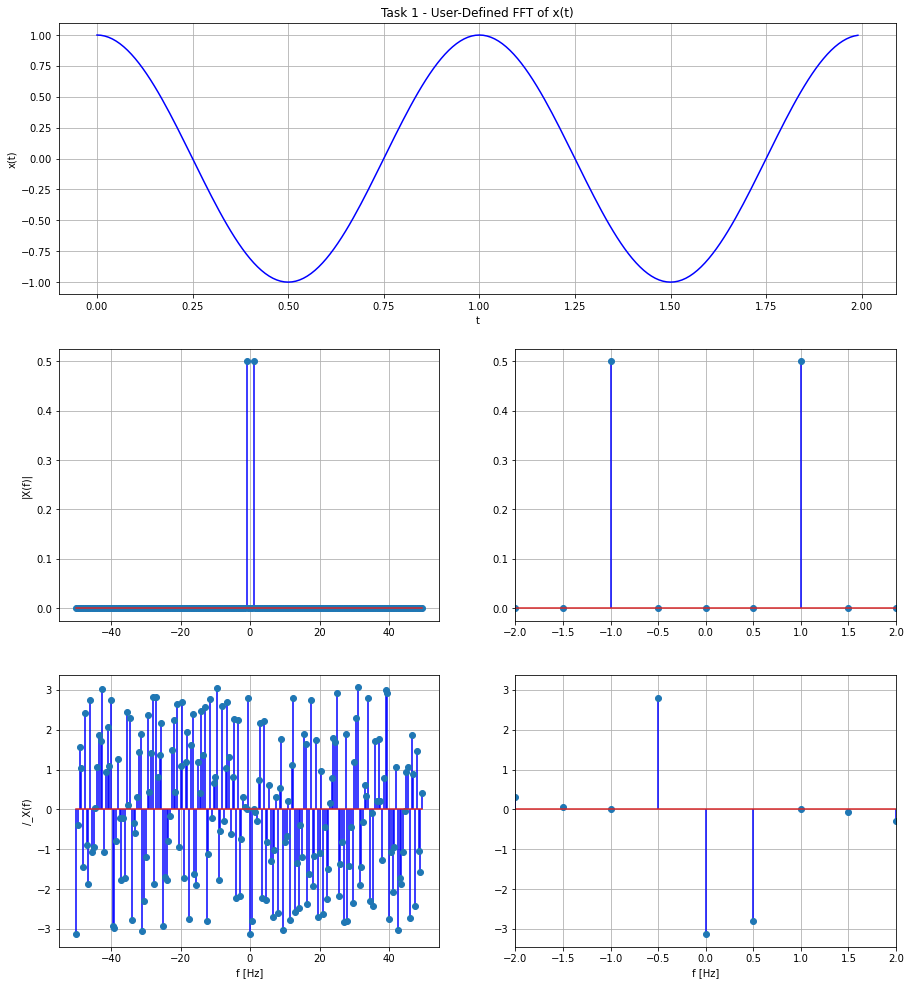
\includegraphics[width=\linewidth]{p1t1.png}
  \caption{Function and FFT Results of Equation \eqref{eq: 1}}
  \label{fig: p1t1}
\end{figure}
\begin{figure}[h!]
  \centering
  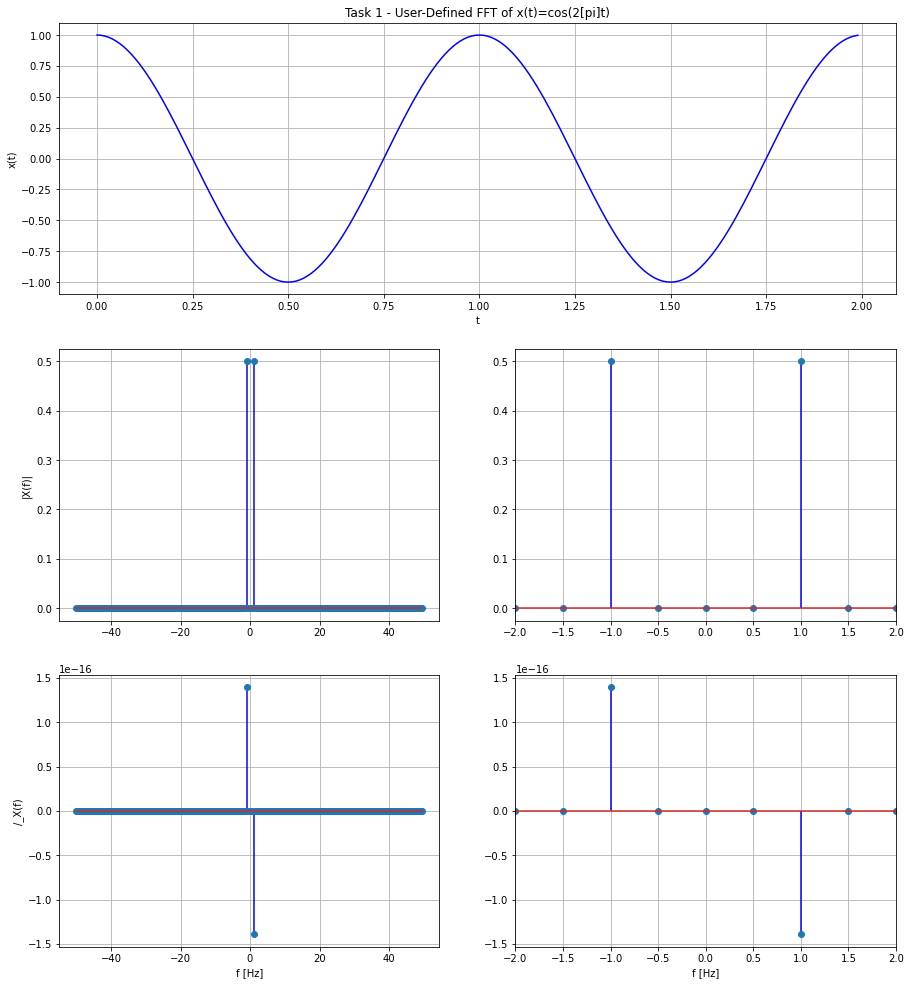
\includegraphics[width=\linewidth]{p1t1f.png}
  \caption{Function and FFT Results of Equation \eqref{eq: 1} (Filtered)}
  \label{fig: p1t1f}
\end{figure}
\begin{figure}[h!]
  \centering
  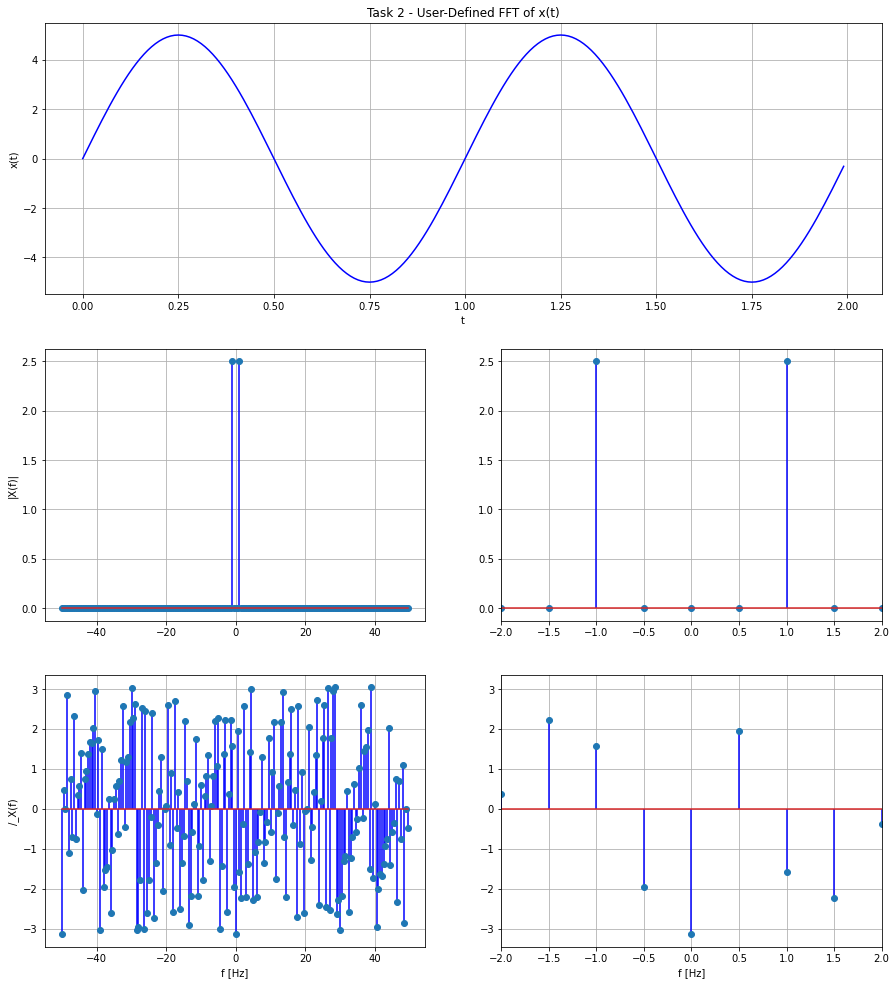
\includegraphics[width=\linewidth]{p1t2.png}
  \caption{Function and FFT Results of Equation \eqref{eq: 2}}
  \label{fig: p1t2}
\end{figure}
\begin{figure}[h!]
  \centering
  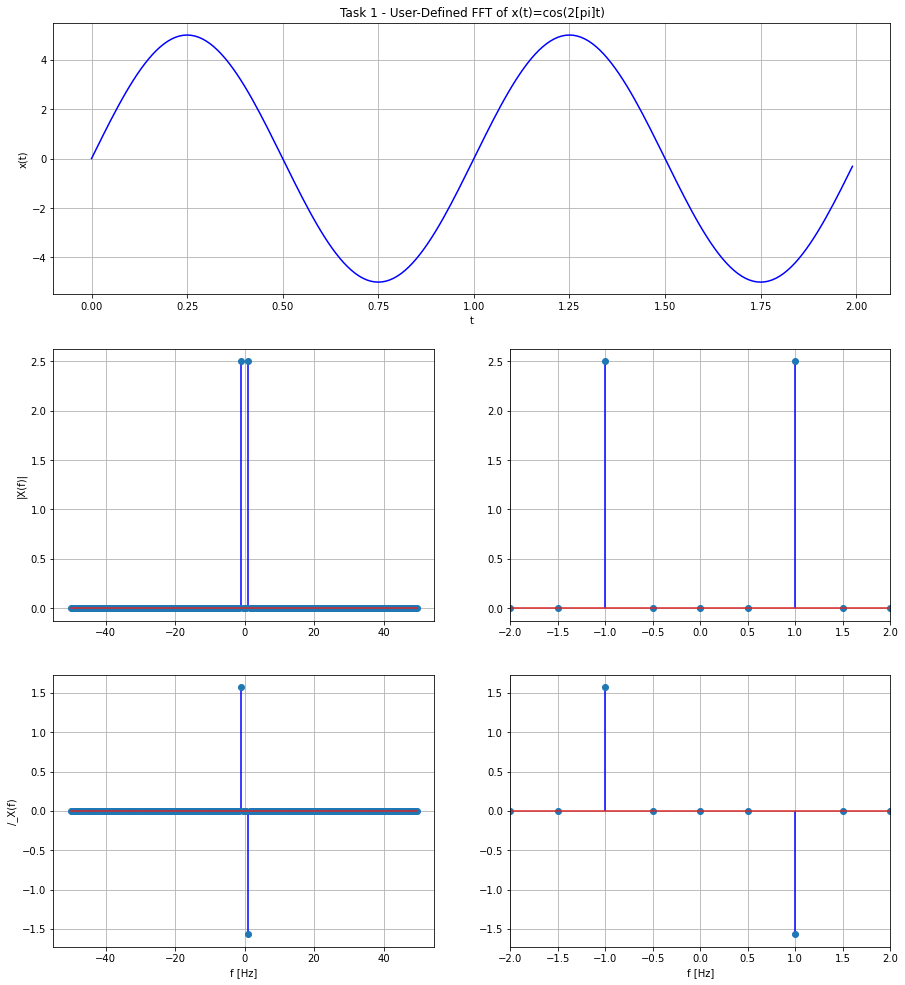
\includegraphics[width=\linewidth]{p1t2f.png}
  \caption{Function and FFT Results of Equation \eqref{eq: 2} (Filtered)}
  \label{fig: p1t2f}
\end{figure}
\begin{figure}[h!]
  \centering
  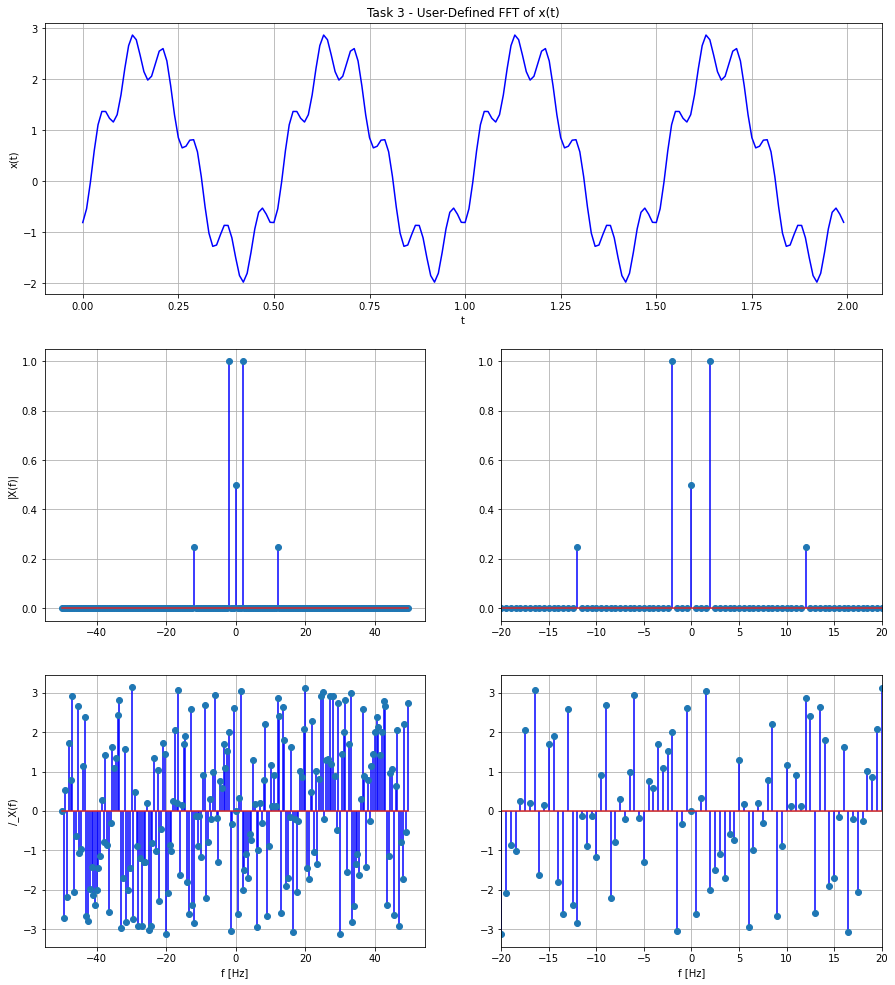
\includegraphics[width=\linewidth]{p1t3.png}
  \caption{Function and FFT Results of Equation \eqref{eq: 3}}
  \label{fig: p1t3}
\end{figure}
\begin{figure}[h!]
  \centering
  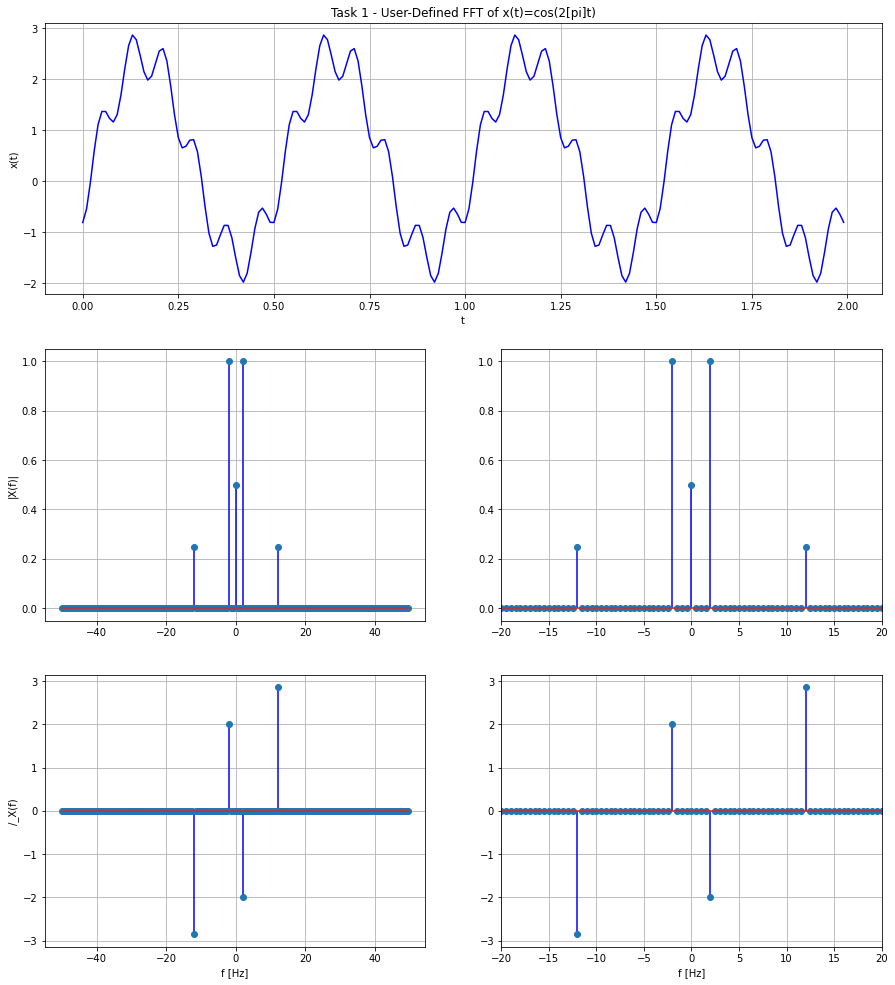
\includegraphics[width=\linewidth]{p1t3f.png}
  \caption{Function and FFT Results of Equation \eqref{eq: 3} (Filtered)}
  \label{fig: p1t3f}
\end{figure}
\begin{figure}[h!]
  \centering
  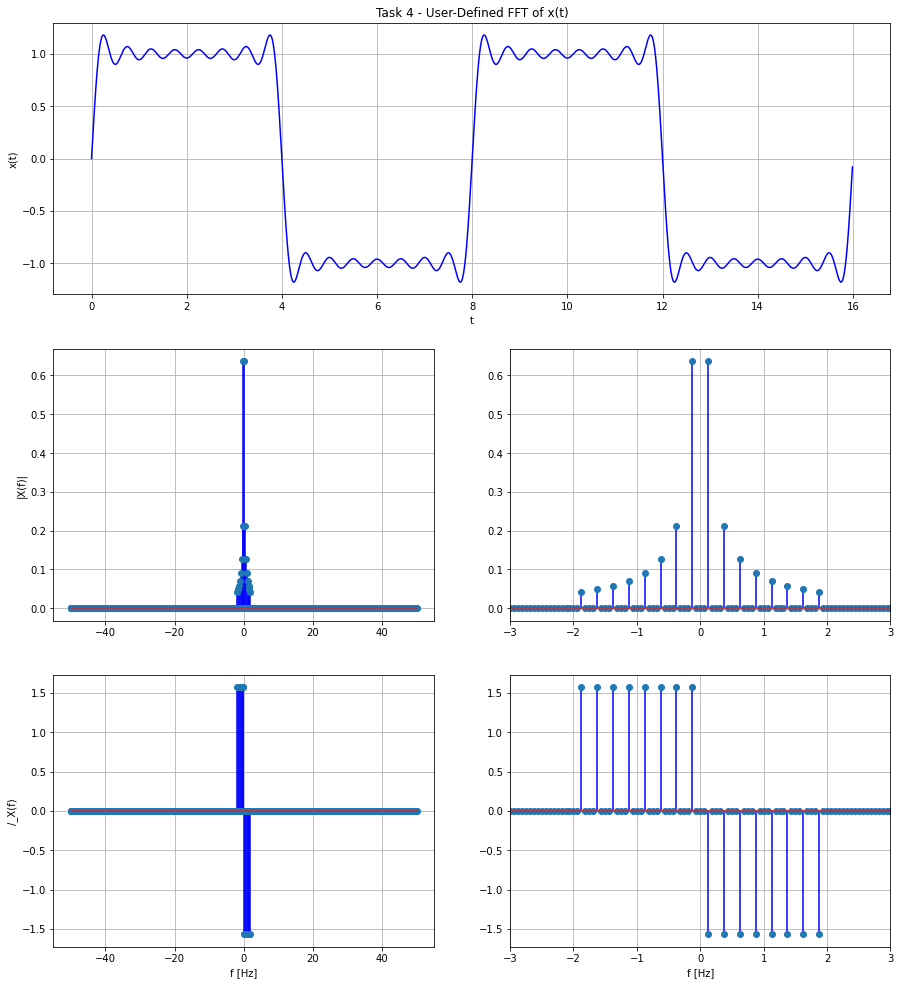
\includegraphics[width=\linewidth]{p1t5.png}
  \caption{Function and FFT Results of Equation \eqref{eq: 4} (Filtered)}
  \label{fig: p1t5}
\end{figure}


\section{Error Analysis}\label{section: ErAn}
One consideration in sources of error in this lab is the Fast Fourier Transform itself. As the name might imply, this is an approximation algorithm to find the fourier transform
of a function and is not exact as compared to the Theoretical Fourier Transform of a function. See \nameref{section: Questions} Section for further discussion (Question 3).1
\section{Questions}\label{section: Questions}
\begin{enumerate}
  \item What happens if \texttt{fs} is lower? If it is higher?
  \begin{itemize}
    \item As \texttt{fs} is the the sampling frequency, the greater it is the more resolution there will be in the output of the FFT. Thus, if it is lower the resolution
    would be lower. The more samples you have the more accurate your results should be, so a very complicated function may benefit from a higher \texttt{fs} value.
  \end{itemize}
  \item What difference does eliminating the small phase magnitude make?
  \begin{itemize}
    \item When the small phase magnitude is eliminated (\texttt{x\_mag < 10e-10}), it is like filtering the results to only view what is important. As the angle for the
    very small magnitude terms exists, it is still shown on the angle plots. But, as the magnitude of of majority of the terms is insignificant the angle of the final 
    function will have an insignificant amount of attenuation from terms with such a small magnitude.
  \end{itemize}
  \item Verify your results from \textbf{Tasks 1 and 2} using the Fourier transforms of cosine and sine. Explain why your results are correct.
  \begin{itemize}
    \item Fourier Transform in Hz of \textbf{Cosine}: $\frac{1}{2}[\delta(f+f_0) + \delta(f-f_0)]$ ;\textbf{Sine}: $\frac{j}{2}[\delta(f+f_0) - \delta(f-f_0)]$. We can see the magnitude and angle will match Plots \ref{fig: p1t1f} \& \ref{fig: p1t2f}
    when substituting in Equations \eqref{eq: 1} \& \eqref{eq: 2}.
  \end{itemize}
  \item Leave any feedback on the clarity of lab tasks, expectations, and deliverables.
  \begin{itemize}
    \item This lab was very clear for all instructions, expectations and deliverables.
  \end{itemize}
\end{enumerate}
\section{Conclusion}
In conclusion, I feel this lab was very successful. It would have been nice if the lab talked further about how FFT theory, but this is something students can always look into
themselves. All in all, I am very satisfied with what this lab has taught me and feel it was an 
excellent use of time.
\newpage
\thispagestyle{customblank}
\section{Attachments}\label{section: Attachments}
No attachments for this lab.
% \centering\begin{enumerate}
%   \item Pre-Lab
% \end{enumerate}
\vspace*{\fill}

% 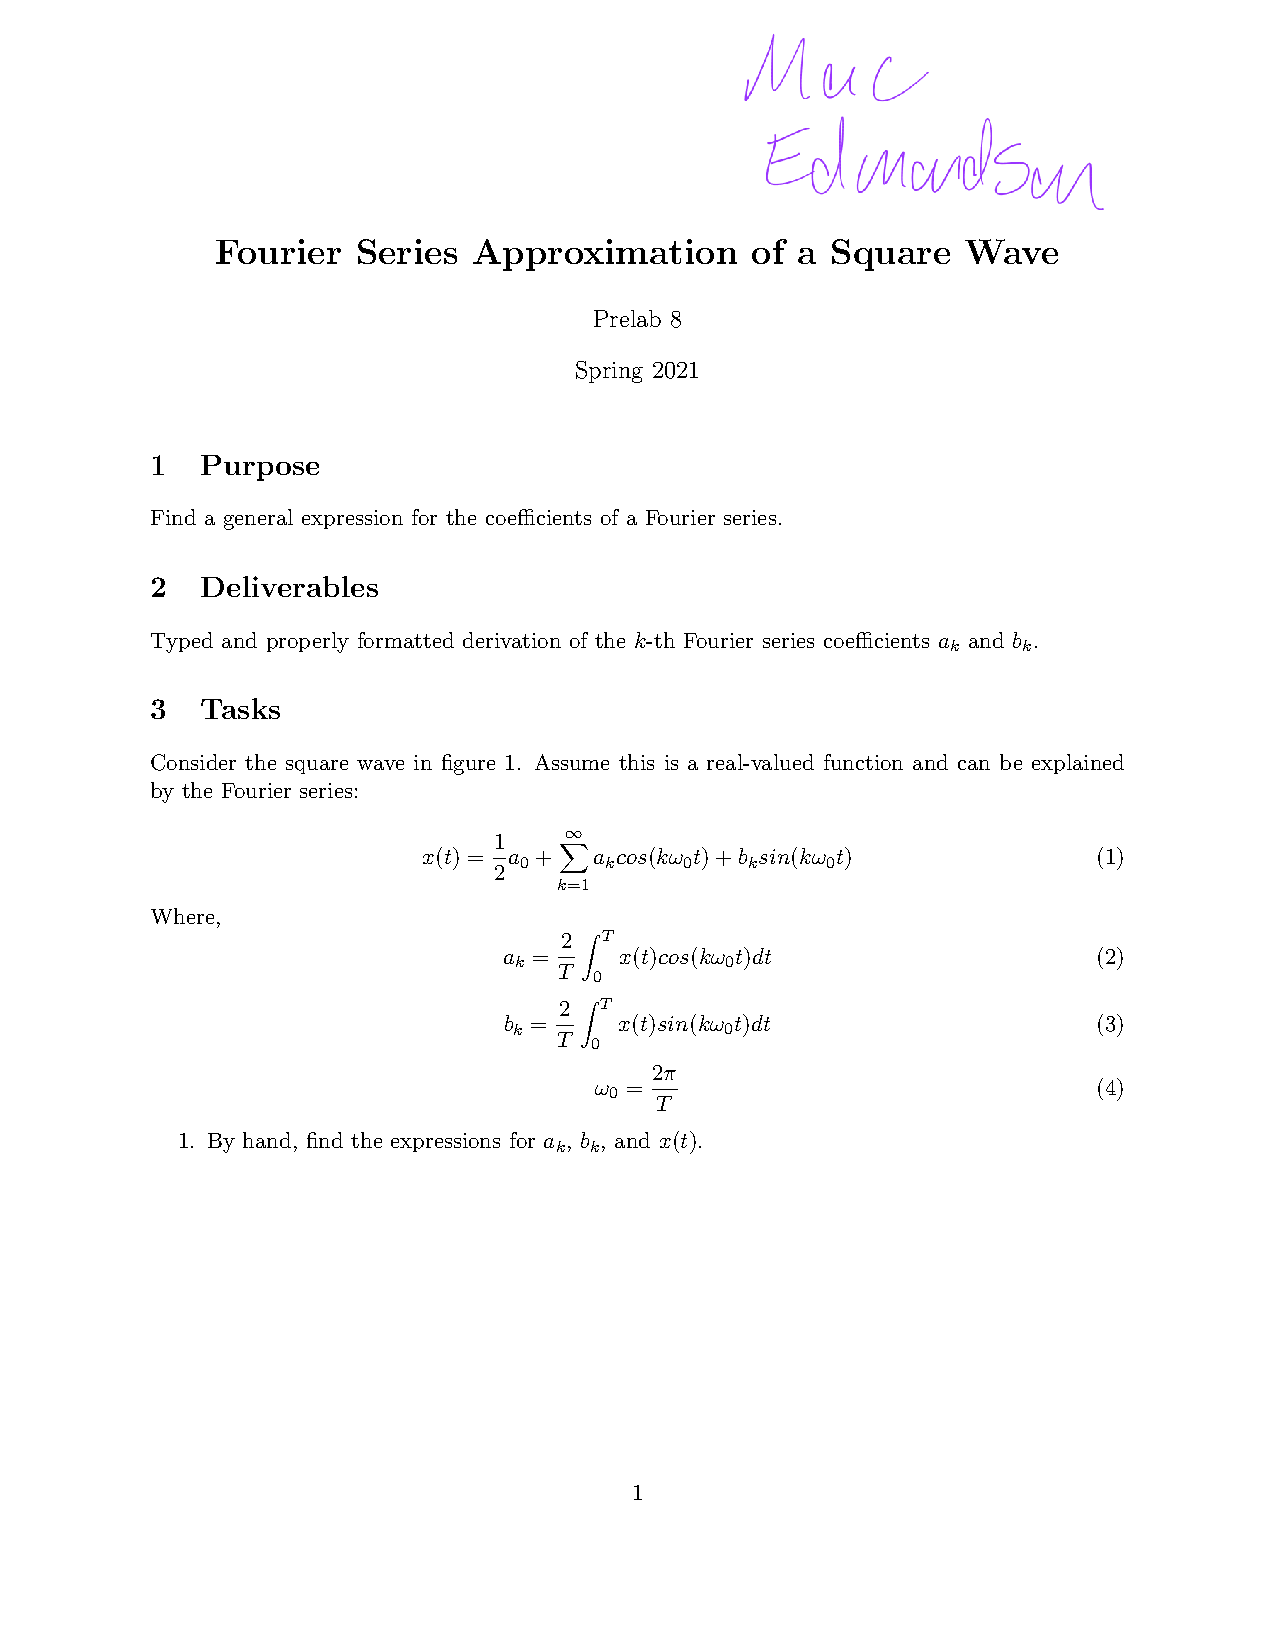
\includepdf[pages=-, offset=1in -1in]{./attachments/lab8_pre.pdf}
% \includepdf[pages=3, offset=1in -1in]{./attachments/lab5.pdf}

% \begin{thebibliography}{111} 
% \thispagestyle{customplain}

% \end{thebibliography}
\end{document}
%This template was created by Roza Aceska.